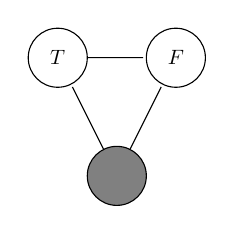
\begin{tikzpicture}[shorten >=1pt,node distance=2cm,auto,scale=1.5,nd/.style={draw=black,circle,scale=\sc,minimum width=0.75 cm,minimum height=1 cm},ndg/.style={nd,fill=gray}]
\def\sc{0.75}
\node[ndg] (R30) at (0.5,3) {};
\node[nd]  (R40) at (0,4)   {$T$};
\node[nd]  (R41) at (1,4)   {$F$};
\foreach \i/\j in {30/40,30/41,40/41} {
  \path (R\i) edge (R\j);
}
\end{tikzpicture}